% Copyright © 2012-2013 Martin Ueding <dev@martin-ueding.de>
%
% Copyright © 2012 Martin Ueding <dev@martin-ueding.de>
%
\documentclass[11pt, ngerman, fleqn]{scrartcl}

\usepackage{graphicx}

%%%%%%%%%%%%%%%%%%%%%%%%%%%%%%%%%%%%%%%%%%%%%%%%%%%%%%%%%%%%%%%%%%%%%%%%%%%%%%%
%                                Locale, date                                 %
%%%%%%%%%%%%%%%%%%%%%%%%%%%%%%%%%%%%%%%%%%%%%%%%%%%%%%%%%%%%%%%%%%%%%%%%%%%%%%%

\usepackage{babel}
\usepackage[iso]{isodate}

%%%%%%%%%%%%%%%%%%%%%%%%%%%%%%%%%%%%%%%%%%%%%%%%%%%%%%%%%%%%%%%%%%%%%%%%%%%%%%%
%                          Margins and other spacing                          %
%%%%%%%%%%%%%%%%%%%%%%%%%%%%%%%%%%%%%%%%%%%%%%%%%%%%%%%%%%%%%%%%%%%%%%%%%%%%%%%

\usepackage[activate]{pdfcprot}
\usepackage[left=3cm, right=2cm, top=2cm, bottom=2cm]{geometry}
\usepackage[parfill]{parskip}
\usepackage{setspace}

\setlength{\columnsep}{2cm}

%%%%%%%%%%%%%%%%%%%%%%%%%%%%%%%%%%%%%%%%%%%%%%%%%%%%%%%%%%%%%%%%%%%%%%%%%%%%%%%
%                                    Color                                    %
%%%%%%%%%%%%%%%%%%%%%%%%%%%%%%%%%%%%%%%%%%%%%%%%%%%%%%%%%%%%%%%%%%%%%%%%%%%%%%%

\usepackage{color}

\definecolor{darkblue}{rgb}{0,0,.5}
\definecolor{darkgreen}{rgb}{0,.5,0}
\definecolor{darkred}{rgb}{.7,0,0}

%%%%%%%%%%%%%%%%%%%%%%%%%%%%%%%%%%%%%%%%%%%%%%%%%%%%%%%%%%%%%%%%%%%%%%%%%%%%%%%
%                         Font and font like settings                         %
%%%%%%%%%%%%%%%%%%%%%%%%%%%%%%%%%%%%%%%%%%%%%%%%%%%%%%%%%%%%%%%%%%%%%%%%%%%%%%%

\usepackage[charter, greekuppercase=italicized]{mathdesign}
\usepackage{beramono}
\usepackage{berasans}

% Style of vectors and tensors.
\newcommand{\tens}[1]{\boldsymbol{\mathsf{#1}}}
\renewcommand{\vec}[1]{\boldsymbol{#1}}

%%%%%%%%%%%%%%%%%%%%%%%%%%%%%%%%%%%%%%%%%%%%%%%%%%%%%%%%%%%%%%%%%%%%%%%%%%%%%%%
%                               Input encoding                                %
%%%%%%%%%%%%%%%%%%%%%%%%%%%%%%%%%%%%%%%%%%%%%%%%%%%%%%%%%%%%%%%%%%%%%%%%%%%%%%%

\usepackage[T1]{fontenc}
\usepackage[utf8]{inputenc}

%%%%%%%%%%%%%%%%%%%%%%%%%%%%%%%%%%%%%%%%%%%%%%%%%%%%%%%%%%%%%%%%%%%%%%%%%%%%%%%
%                         Hyperrefs and PDF metadata                          %
%%%%%%%%%%%%%%%%%%%%%%%%%%%%%%%%%%%%%%%%%%%%%%%%%%%%%%%%%%%%%%%%%%%%%%%%%%%%%%%

\usepackage{hyperref}
\usepackage{lastpage}

\hypersetup{
	breaklinks=false,
	citecolor=darkgreen,
	colorlinks=true,
	linkcolor=black,
	menucolor=black,
	pdfauthor={Martin Ueding},
	urlcolor=darkblue,
}

%%%%%%%%%%%%%%%%%%%%%%%%%%%%%%%%%%%%%%%%%%%%%%%%%%%%%%%%%%%%%%%%%%%%%%%%%%%%%%%
%                               Math Operators                                %
%%%%%%%%%%%%%%%%%%%%%%%%%%%%%%%%%%%%%%%%%%%%%%%%%%%%%%%%%%%%%%%%%%%%%%%%%%%%%%%

\usepackage[thinspace, squaren]{SIunits}
\usepackage{amsmath}
\usepackage{amsthm}
\usepackage{commath}

% Word like operators.
\DeclareMathOperator{\acosh}{arcosh}
\DeclareMathOperator{\arcosh}{arcosh}
\DeclareMathOperator{\arcsinh}{arsinh}
\DeclareMathOperator{\arsinh}{arsinh}
\DeclareMathOperator{\asinh}{arsinh}
\DeclareMathOperator{\card}{card}
\DeclareMathOperator{\diam}{diam}
\renewcommand{\Im}{\mathop{{}\mathrm{Im}}\nolimits}
\renewcommand{\Re}{\mathop{{}\mathrm{Re}}\nolimits}

% Special single letters.
\DeclareMathOperator{\fourier}{\mathcal{F}}
\newcommand{\C}{\ensuremath{\mathbb C}}
\newcommand{\ee}{\mathrm e}
\newcommand{\ii}{\mathrm i}
\newcommand{\N}{\ensuremath{\mathbb N}}
\newcommand{\R}{\ensuremath{\mathbb R}}
\newcommand{\Z}{\ensuremath{\mathbb Z}}

% Shape like operators.
\DeclareMathOperator{\dalambert}{\Box}
\DeclareMathOperator{\laplace}{\bigtriangleup}
\newcommand{\curl}{\vnabla \times}
\newcommand{\divergence}[1]{\inner{\vnabla}{#1}}
\newcommand{\vnabla}{\vec \nabla}

% Shortcuts
\newcommand{\ev}{\hat{\vec e}}
\newcommand{\e}[1]{\cdot 10^{#1}}
\newcommand{\half}{\frac 12}
\newcommand{\inner}[2]{\left\langle #1, #2 \right\rangle}

% Placeholders.
\newcommand{\emesswert}{\del{\messwert \pm \messwert}}
\newcommand{\fehlt}{\textcolor{darkred}{Hier fehlen noch Inhalte.}\marginpar{\textcolor{darkred}{!}}}
\newcommand{\messwert}{\textcolor{blue}{\square}}
\newcommand{\punkte}{\textcolor{white}{xxxxx}}

%%%%%%%%%%%%%%%%%%%%%%%%%%%%%%%%%%%%%%%%%%%%%%%%%%%%%%%%%%%%%%%%%%%%%%%%%%%%%%%
%                                  Headings                                   %
%%%%%%%%%%%%%%%%%%%%%%%%%%%%%%%%%%%%%%%%%%%%%%%%%%%%%%%%%%%%%%%%%%%%%%%%%%%%%%%

\usepackage{scrpage2}

\pagestyle{scrheadings}

\automark{section}
\cfoot{\footnotesize{Seite \thepage\ / \pageref{LastPage}}}
\chead{}
\ihead{}
\ohead{\rightmark}
\setheadsepline{.4pt}


\usepackage{tikz}

\newcommand{\themodul}{physik321}
\newcommand{\thegruppe}{Gruppe 8 -- Julia Volmer}
\newcommand{\theuebung}{12}

\ifoot{\footnotesize{Martin Ueding, Simon Schlepphorst}}
\ihead{\themodul{} -- Übung \theuebung}
\ofoot{\footnotesize{\thegruppe}}

\def\thesection{H \theuebung.\arabic{section}}
\def\thesubsubsection{\thesubsection\alph{section}}

\title{\themodul{} -- Übung \theuebung \\ \vspace{0.5cm} \large{\thegruppe}}

\author{
	Martin Ueding \\ \small{\href{mailto:mu@uni-bonn.de}{mu@uni-bonn.de}}
	\and
	Simon Schlepphorst \\ \small{\href{mailto:s2@uni-bonn.de}{s2@uni-bonn.de}}
}

\hypersetup{
	pdftitle={\themodul {} - Übung \theuebung},
}

\begin{document}

\maketitle

\begin{table}[h]
	\centering
	\begin{tabular}{l|c|c|c|c|c|c}
		Aufgabe
		& \ref 1
		& \ref 2
		& \ref 3
		& \ref 4
		& \ref 5
		& $\sum$   \\
		\hline
		Punkte
		& \punkte / 20
		& \punkte / 20
		& \punkte / 10
		& \punkte / 25
		& \punkte / 15
		& \punkte / 50
	\end{tabular}
\end{table}

%%%%%%%%%%%%%%%%%%%%%%%%%%%%%%%%%%%%%%%%%%%%%%%%%%%%%%%%%%%%%%%%%%%%%%%%%%%%%%%
%                            der Feldstärketensor                            %
%%%%%%%%%%%%%%%%%%%%%%%%%%%%%%%%%%%%%%%%%%%%%%%%%%%%%%%%%%%%%%%%%%%%%%%%%%%%%%%

\section{der Feldstärketensor}
\label 1

\subsection{Lorenzeichung}

Wir beginnen mit den inhomogenen Maxwellgleichungen:
\begin{gather*}
	\divergence{\vec E} = \frac{1}{\varepsilon_0} \rho \\
	\curl \vec B - \frac{1}{c^2} \dot{\vec E} = \mu_0 \vec j
\end{gather*}

Dort setzen wir die Beziehungen $\vec E = - \vnabla \phi - \dot{\vec A}$ und
$\vec B = \curl \vec A$ ein. Wir erhalten:
\begin{gather*}
	- \vnabla \phi - \divergence{\dot{\vec A}} = \frac{1}{\varepsilon_0} \rho \\
	\curl \curl \vec A + \frac 1{c^2} \laplace \dot \phi + \frac 1{c^2} \ddot{\vec A} = \mu_0 \vec j
\end{gather*}

Wir benutzen $\curl \curl \vec A = \vnabla \divergence{\vec A} - \laplace \vec
A$ und erhalten:
\begin{gather*}
	- \vnabla \phi - \dpd{}t \divergence{\vec A} = \frac{1}{\varepsilon_0} \rho \\
	\dalambert A + \vnabla\del{\divergence{\vec A} + \frac 1{c^2} \dot \phi} = \mu_0 \vec j
\end{gather*}

Nun wenden wir die Lorenzeichung $\phi/\del{c^2} + \divergence{\vec A} = 0$ auf
beide Gleichungen an:
\begin{gather*}
	\dalambert \phi = \frac{1}{\varepsilon_0} \rho \\
	\dalambert \vec A = \mu_0 \vec j
\end{gather*}

Mit $\phi/c = A^0$ und $\del{\vec A}^i = A^i$ erhalten wir $\dalambert A^\mu =
\mu_0 j^\mu$.

\subsection{Vierervektor und Inertialsystem}

$\dalambert$ ist durch ein Skalarprodukt definiert, also invariant. $\tens j$
ist als Vierervektor invariant. Die Konstante $\mu_0$ ist ein Skalar und
ebenfalls invariant. Somit muss $\tens A$ auch invariant sein.

Die Lorenzeichung funktioniert in jedem Inertialsystem, weil sie durch ein
invariantes Skalarprodukt, $\partial_\mu A^\mu$, definiert ist.

\subsection{Feldstärketensor}

Die Felder sind wie folgt durch die Potentiale definiert:
\begin{gather*}
	\vec E = - \vnabla \phi - \dot{\vec A} \\
	\vec B = \curl \vec A
\end{gather*}

Wir schreiben jeweils die Komponenten von $\vec E$ und $\vec B$. Dabei benutzen
wir im zweiten Schritt aus, dass $\partial_i = - \partial^i$ ist, jedoch
$\partial_0 = \partial^0$.
\begin{gather*}
	E_1
	= - \partial_1 A^0 - \partial_0 A^1
	= \partial^1 A^0 - \partial^0 A^1
	\\
	E_2
	= - \partial_2 A^0 - \partial_0 A^2
	= \partial^2 A^0 - \partial^0 A^2
	\\
	E_3
	= - \partial_3 A^0 - \partial_0 A^3
	= \partial^3 A^0 - \partial^0 A^3
	\\
	B_1
	= \partial_2 A^3 - \partial_3 A^2
	= -\del{\partial^2 A^3 - \partial^3 A^2}
	\\
	B_2
	= \partial_3 A^1 - \partial_1 A^3
	= \del{\partial^3 A^1 - \partial^1 A^3}
	\\
	B_3
	= \partial_1 A^2 - \partial_2 A^1
	= \del{\partial^1 A^2 - \partial^2 A^1}
	\\
\end{gather*}

An diesem Schritt kann man den Vorgang gut in der Penrose-Notation
\cite{penrose-road_to_reality} darstellen.  Dabei ist der Vierervektor $\tens
A$:
\begin{center}
	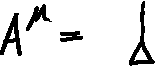
\includegraphics{H1-Penrose-2-crop.pdf}
\end{center}

Wir bauen aus dem Vierervektor $\tens A$ und der kovarianten Ableitung (der
perfekte Kreis) einen Tensor $\tens F$ von Stufe ${2 \brack 0}$ zusammen. Dabei
führen wir noch Antisymmetrie in den beiden Indizes $\mu$ und $\nu$ durch den
fetten Balken ein. Diese definieren wir in der idempotenten Form als $x^{[a}
y^{b]} := \half \del{x^a y^b - x^b y^a}$. In Indexschreibweise ist der
Feldstärketensor:
\[
	2 \partial^{[\mu} A^{\nu]} := \partial^\mu A^\nu - \partial^\nu A^\mu
\]
\begin{center}
	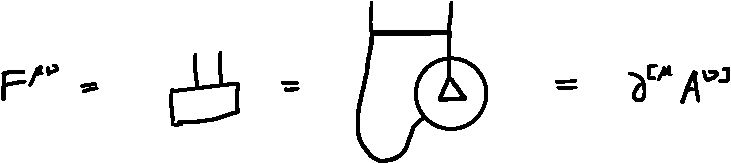
\includegraphics{H1-Penrose-1-crop.pdf}
\end{center}

Als Matrix dargestellt erhalten wir das, was auf dem Aufgabenblatt angegeben
ist:
\[
	\tens F
	=
	\begin{pmatrix}
		0 & -E_1/c & -E_1/c & -E_1/c \\
		E_1/c & 0 & -B_3 & B_2 \\
		E_2/c & B_3 & 0 & -B_1 \\
		E_3/c & -B_2 & B_1 & 0 \\
	\end{pmatrix}
\]

In der Diagrammnotation oder in der Schreibweise $\partial^{[\mu} A^{\nu]}$, als
auch in der Matrixschreibweise, erkennen wir, dass der Tensor antisymmetrisch
ist. Daher muss er nicht nur spurlos, sondern auf der ganzen Diagonalen
$F^{\mu\mu} = 0$ sein.

\subsection{Transformationseigenschaften}

\paragraph{Transformation}

Als Tensor der Stufe ${2 \brack 0}$ wird dieser mit zwei normalen
Transformationen transformiert:
\[
	F^{\mu\nu} \mapsto \Lambda^\mu{}_\alpha \Lambda^\nu{}_\beta F^{\alpha\beta}
\]

In der Diagrammnotation ist dies direkt zu sehen:
\begin{center}
	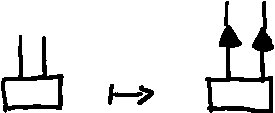
\includegraphics{H1-Penrose-9-crop.pdf}
\end{center}

\paragraph{nicht Teil eines Vierervektors}

Angenommen, wir könnten $\vec B$ als Vierervektor $\tens B$ schreiben durch:
\[
	B^\mu = F^{\mu0}
\]

Dann müsste $\tens E$ sich als Vierervektor transformieren lassen, also einfach
kontravariant. $\tens F$ transformiert sich \emph{zweifach} kontravariant. Nach
Anwendung der Transformation $\tens \Lambda$ ist diese Gleichung nicht mehr zu
halten:
\[
	E'^\mu
	= \Lambda^\mu{}_\nu E^\nu
	\neq
	\Lambda^\mu{}_\alpha \Lambda^0{}_\beta F^{\alpha\beta}
	= F'^{\mu0}
\]

Durch die Transformation von $\tens F$ entstehen Mischterme mit $B_i$, die in
einem reinen Vierervektor $\tens E$ nicht auftreten würden. Analog gilt dies
für einen Vierervektor $\tens B$, den man auch $\hat{\tens F}$ erzeugen könnte.

\subsection{zweifach kovarianter Tensor}

Die beiden Indizes von $\tens F$ können wir mit dem metrischen Tensor
herunterziehen.
\begin{center}
	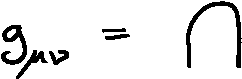
\includegraphics{H1-Penrose-5-crop.pdf}
\end{center}

So erhalten wir $F_{\mu\nu} = g_{\mu\alpha} g_{\nu\beta} = F^{\alpha\beta}$:
\begin{center}
	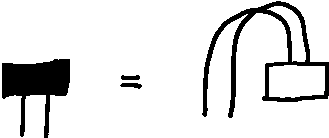
\includegraphics{H1-Penrose-10-crop.pdf}
\end{center}

Dabei sorgt der erste metrische Tensor auf $\mu$ dafür, dass die Vorzeichen in
den Zeilen 1 bis 3 gedreht werden. Dann kehrt das zweite $\tens g$ die
Vorzeichen in den Spalten 1 bis 3 um. Es werden nur die Vorzeichen
von $F^{0i}$ und $F^{i0}$ gedreht. Somit wechseln nur die Terme des
elektrischen Feldes das Vorzeichen und wir erhalten:
\[
	\tens F
	=
	\begin{pmatrix}
		0 & E_1/c & E_1/c & E_1/c \\
		-E_1/c & 0 & -B_3 & B_2 \\
		-E_2/c & B_3 & 0 & -B_1 \\
		-E_3/c & -B_2 & B_1 & 0 \\
	\end{pmatrix}
\]

\subsection{dualer Feldstärketensor}

Wir wenden den $\tens\epsilon$-Tensor
\begin{center}
	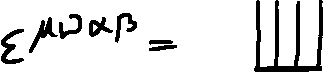
\includegraphics{H1-Penrose-4-crop.pdf}
\end{center}
auf den kovarianten Feldstärketensor an:
\begin{center}
	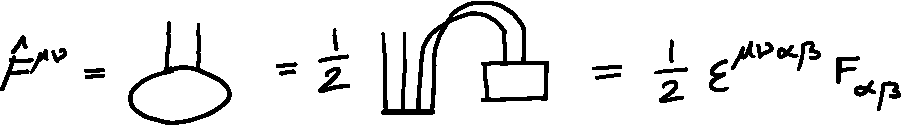
\includegraphics{H1-Penrose-3-crop.pdf}
\end{center}

Dabei wollen wir exemplarisch den Eintrag $\hat F^{01}$ berechnen, die weiteren
Einträge berechnen sich ähnlich. Dieser Eintrag ist:
\[
	\hat F^{01} = \half \epsilon^{01\alpha\beta} F_{\alpha\beta}
\]

Es gibt zwei Kombinationen für $\alpha$ und $\beta$, so dass nicht null
herauskommt, einmal $(2, 3)$ und $(3, 2)$. Dabei ist $F^{23} = -B_2$ und
$F^{32} = B_2$ (Antisymmetrie). Die Differenz der beiden ergibt $-2 B_2$, durch
das $1/2$ erhalten wir genau $-B_2$.

Dies können wir für alle Elemente von $\hat{\tens F}$ machen und erhalten so
den kompletten Tensor.

\subsection{homogene Maxwellgleichungen}

Wir bilden die kovariante Ableitung und kontrahieren diese mit dem dualen
Feldstärketensor:
\begin{center}
	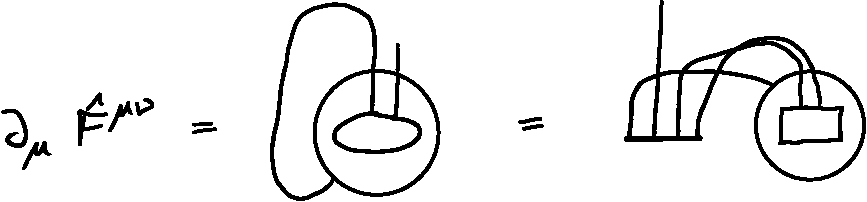
\includegraphics{H1-Penrose-6-crop.pdf}
\end{center}

Dabei gehen wir die Komponenten einzeln durch:
\begin{description}
	\item[Fall $\nu = 0$]
		\[
			\partial_\mu \hat F^{\mu 0}
			=
			\partial_\mu
			\begin{pmatrix}
				0 \\ -B_1 \\ -B_2 \\ -B_3
			\end{pmatrix}^\mu
			=
			\partial_i B^i = 0
		\]

	\item[Fall $\nu = 1$]
		\[
			\partial_\mu \hat F^{\mu 1}
			=
			\partial_\mu
			\begin{pmatrix}
				B_1 \\ 0 \\ E_3/c \\ -E_2/c
			\end{pmatrix}^\mu
			= c \dot B_1 + \frac 1c \del{\partial_2 E_3 - \partial_3 E_2}
			= 0
		\]

	\item[Fall $\nu = 2$]
		\[
			\partial_\mu \hat F^{\mu 2}
			=
			\partial_\mu
			\begin{pmatrix}
				B_2 \\ -E_3/c \\ 0 \\ E_1/c
			\end{pmatrix}^\mu
			= c \dot B_2 + \frac 1c \del{\partial_3 E_1 - \partial_1 E_3}
			= 0
		\]

	\item[Fall $\nu = 3$]
		\[
			\partial_\mu \hat F^{\mu 3}
			=
			\partial_\mu
			\begin{pmatrix}
				B_3 \\ E_2/c \\ -E_1/c \\ 0
			\end{pmatrix}^\mu
			= c \dot B_3 + \frac 1{c} \del{\partial_1 E_2 - \partial_2 E_1}
			= 0
		\]
\end{description}

Wir kombinieren alle vier Gleichungen und erhalten die inhomogenen
Maxwellgleichungen:
\[
	\divergence{\vec B} = 0
	\eqnsep
	\curl \vec E + \frac 1{c^2} \dot{\vec B} = 0
\]

Um die Gleichungen nur mit $F^{\mu\nu}$ auszudrücken, setzen wir die Definition
von $\hat F^{\mu\nu}$ ein:
\[
	\partial_\mu \hat F^{\mu\nu}
	= \half \partial_\mu \epsilon^{\mu\nu\alpha\beta} g_{\alpha\eta} g_{\beta\tau} F^{\eta\tau}
	= 0
\]

Siehe dazu das Bild am Anfang dieser Teilaufgabe.

\subsection{Lorentzinvarianz}

Die Gleichungen hängen davon ab, dass der komplette Ausdruck $\partial_\mu \hat
F^{\mu\nu}$ gerade der Nulltensor ist. Wir wissen, dass Vierervektoren
invariant sind. Im folgenden Bild ist gezeigt, dass der komplette Ausdruck
insgesamt nur eine Transformation (ausgefülltes Dreieck) braucht, um
transformiert zu werden. Alle anderen Transformationen treten mit der
Gegentransformation. Er ist also ein Vierervektor und somit lorentzinvariant.
\begin{center}
	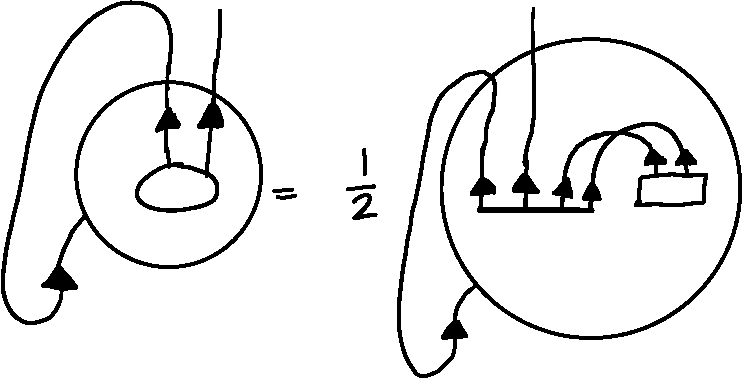
\includegraphics{H1-Penrose-7-crop.pdf}
\end{center}

Auf der anderen Seite der Gleichung dürfte anstelle der 0 auch ein Vierervektor
stehen, dies ist bei den inhomogenen Maxwellgleichungen der Fall.

\subsection{Transformation von $\tens F$ auf $\hat{\tens F}$}

Die Transformation $\tens T$, die $\tens F$ auf $\hat{\tens F}$ abbildet, ist
durch folgendes Konstrukt (ausgefüllter Kreis) gegeben:
\begin{center}
	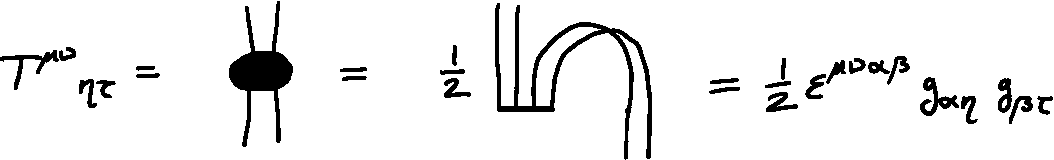
\includegraphics{H1-Penrose-8-crop.pdf}
\end{center}

Dabei ist $\tens T$ ein Tensor der Stufe ${2 \brack 2}$. Dies ist es der
gemischte $\tens \epsilon$-Tensor $\half \epsilon^{\mu\nu}{}_{\alpha\beta}$.

%%%%%%%%%%%%%%%%%%%%%%%%%%%%%%%%%%%%%%%%%%%%%%%%%%%%%%%%%%%%%%%%%%%%%%%%%%%%%%%
%                   Energie des elektromagnetischen Feldes                    %
%%%%%%%%%%%%%%%%%%%%%%%%%%%%%%%%%%%%%%%%%%%%%%%%%%%%%%%%%%%%%%%%%%%%%%%%%%%%%%%

\section{Energie des elektromagnetischen Feldes}
\label 2

\subsection{Transformations- und Symmetrieeigenschaften}

Der Energie-Impuls-Tensor (Rechteck mit Punkt) ist definiert über den
Feldstärketensor (Rechteck) als:
\begin{center}
	\includegraphics{H2-Penrose-1-crop.pdf}
\end{center}

\paragraph{Transformationseigenschaften}

Dieser Tensor transformiert wie jeder andere Tensor der Stufe ${2 \brack 0}$,
man braucht zwei normale Transformationen $\tens \Lambda$.

\paragraph{Symmetrie}

Der Tensor ist symmetrisch. Wir haben einen der beiden Feldstärketensoren mit
einer schwarzen Ecke gekennzeichnet, um die Schritte zu verdeutlichen. Wir
vertauschen die beiden Indizes ($\mapsto$). Dann verschieben wir die beiden
Tensoren ein wenig (erstes $=$). Dann benutzen wir die Antisymmetrie zweimal
(zweites $=$). Wir verschieben wieder (zweite Zeile). Der Tensor mit Indizes
oben (kontravariant), dessen Indizes nach unten gebogen werden, hatten wir
bereits mit dem Tensor mit Indizes unten (kovariant) identifiziert. Somit
erhalten wir den letzten Schritt.
\begin{center}
	\includegraphics{H2-Penrose-7-crop.pdf}
\end{center}

Der metrische Tensor im zweiten Summanden ist symmetrisch, da er Diagonalform
hat.
\begin{center}
	\includegraphics{H2-Penrose-6-crop.pdf}
\end{center}

\paragraph{Spur}

Um die Spur zu bestimmen, kontrahieren wir die beiden verbleibenden Indizes.
Dabei brauchen wir noch einen metrischen Tensor um einen der Indizes
herunterziehen. Wir rechnen diese Aufgabe komplett in der Diagrammnotation.

Zuerst kontrahieren wir den ersten Summanden. Durch Verschieben der
Verbindungen erhalten wir die beiden Tensoren über kreuz kontrahiert. Durch die
Antisymmetrie können wir dies „entwirren“ und erhalten das Negative:
\begin{center}
	\includegraphics{H2-Penrose-2-crop.pdf}
\end{center}

Im zweiten Summanden ist bereits der Feldstärketensor mit einem zweiten
kontrahiert. An den metrischen Tensor schließen wir noch einen Kovarianten an
und erhalten $4$ ($g_{\mu\nu} g^{\mu\nu} = 1$):
\begin{center}
	\includegraphics{H2-Penrose-3-crop.pdf}
\end{center}

Zusammen ist die Spur $T^\mu{}_\mu = 0$:
\begin{center}
	\includegraphics{H2-Penrose-4-crop.pdf}
\end{center}

\subsection{Energiedichte und Energiestromdichte}

\paragraph{Energiedichte}

Wir beginnen mit der Energiedichte:
\begin{align*}
	T^{00}
	&= \frac1{\mu_0} g^{0\alpha} F_{\alpha\beta} F^{\beta0} + \frac1{4\mu_0} g^{00} F_{\kappa\lambda} F^{\kappa\lambda} \\
	\intertext{%
		Im ersten Summanden ist durch den metrischen Tensor nur $\alpha = 0$
		interessant. Somit können wir $\tens F$ einsetzen:
	}
	&= \frac1{\mu_0}
	\begin{pmatrix}
		0 \\ \vec E / c
	\end{pmatrix}
	_\beta
	\begin{pmatrix}
		0 \\ \vec E / c
	\end{pmatrix}
	^\beta
	+ \frac1{4\mu_0} F_{\kappa\lambda} F^{\kappa\lambda} \\
	\intertext{%
		Im letzten Term werden die beiden Matrizen aufeinander gelegt,
		elementweise multipliziert und dann alles aufaddiert.
	}
	&= \varepsilon_0 \vec E^2 + \frac1{2\mu_0} \del{- \frac{\vec E^2}{c^2} + \vec B^2} \\
	&= \half \varepsilon_0 \vec E^2 + \frac1{2\mu_0} \vec B^2 \\
	&= \half \del{\inner{\vec D}{\vec E} + \inner{\vec B}{\vec H}}
\end{align*}

\paragraph{Energiestromdichte}

Für die Energiestromdichte gehen wir ähnlich vor. Dabei leiten wir nur $T^{i0}$
her, da $T^{0i}$ aufgrund der Symmetrie gleich ist.
\begin{align*}
	T^{i0}
	&= \frac1{\mu_0} g^{i\alpha} F_{\alpha\beta} F^{\beta0} + \frac1{4\mu_0} g^{i0} F_{\kappa\lambda} F^{\kappa\lambda} \\
	\intertext{%
		Die $g^{i\alpha}$ sind für $\alpha = i \in \set{1, 2, 3}$ genau $-1$. Alle
		$g^{i0}$ sind 0.
	}
	&= - \frac1{\mu_0} F_{i\beta} F^{\beta0} \\
	&= - \frac1{\mu_0}
	\begin{pmatrix}
		- E_1/c & 0 & -B_3 & B_2 \\
		- E_2/c & B_3 & 0 & -B_1 \\
		- E_3/c & -B_2 & B_1 & 0 \\
	\end{pmatrix}_{i\beta}
	\begin{pmatrix}
		0 \\ E_1/c \\ E_2/c \\ E_3/c
	\end{pmatrix}^{\beta}
	\\
	&= \frac1{c\mu_0}
	\begin{pmatrix}
		E_2B_3 - E_3B_2 \\
		E_3B_1 - E_1B_3 \\
		E_1B_2 - E_2B_1
	\end{pmatrix}_i \\
	&= \frac1{c\mu_0} \del{\vec E \times \vec B}_i \\
	&= \frac1{c} \del{\vec E \times \vec H}_i \\
	&= \frac1{c} \vec S_i \\
\end{align*}

\subsection{kovariante Ableitung}

Wir definieren den Strom Vierervektor in der Diagrammnotation:
\begin{center}
	\includegraphics{H2-Penrose-9-crop.pdf}
\end{center}

Wir wollen zeigen, dass gilt:
\[
	\partial_\nu T^{\mu\nu} = - j_\nu F^{\mu\nu}
\]

Dies im Diagramm:
\begin{center}
	\includegraphics{H2-Penrose-8-crop.pdf}
\end{center}

Wir setzen die Definition von $T^{\mu\nu}$ ein und spalten die Summe in zwei
Ableitungen auf:
\begin{center}
	\includegraphics{H2-Penrose-10-crop.pdf}
\end{center}

Für den ersten Summanden wenden wir die Produktregel für Tensoren an:
\begin{center}
	\includegraphics{H2-Penrose-11-crop.pdf}
\end{center}

Der rechte Teil ist:
\[
	\frac1{\mu_0}
	\del{\partial_\alpha F^{\mu}{}_\nu} F^{\nu\alpha}
	+ \frac1{\mu_0}
	F^\mu{}_\alpha \del{\partial_\nu F^{\alpha\nu}}
\]

Für den zweiten Summanden von weiter oben wenden wir ebenfalls die Produktregel
an:
\begin{center}
	\includegraphics{H2-Penrose-12-crop.pdf}
\end{center}

Alles zusammen:
\[
	\partial_\nu T^{\mu\nu}
	=
	\frac1{\mu_0}
	\del{\partial_\alpha F^{\mu}{}_\nu} F^{\nu\alpha}
	+ \frac1{\mu_0}
	F^\mu{}_\alpha \del{\partial_\nu F^{\alpha\nu}}
	+ \frac1{4\mu_0}
	\del{\partial^\mu F_{\alpha\nu}} F^{\alpha\nu}
	+ \frac1{4\mu_0}
	F^{\alpha\nu} \partial^\mu F_{\alpha\nu}
\]

Die beiden letzten Terme sind gleich, wir fassen sie zusammen:
\[
	\partial_\nu T^{\mu\nu}
	=
	\frac1{\mu_0}
	\del{\partial_\alpha F^{\mu}{}_\nu} F^{\nu\alpha}
	+ \frac1{\mu_0}
	F^\mu{}_\alpha \del{\partial_\nu F^{\alpha\nu}}
	+ \frac1{2\mu_0}
	\del{\partial^\mu F_{\alpha\nu}} F^{\alpha\nu}
\]

Wir benutzen die Relation $\partial_\mu F^{\mu\nu} = \mu_0 j^\nu$ im zweiten
Summanden. Außerdem heben und senken wir Indizes im letzten Summanden:
\[
	\partial_\nu T^{\mu\nu}
	=
	\frac1{\mu_0}
	\del{\partial_\alpha F^{\mu}{}_\nu} F^{\nu\alpha}
	- F^{\mu\alpha} j_\alpha
	+ \frac1{2\mu_0}
	\del{\partial^\mu F^{\alpha\nu}} F_{\alpha\nu}
\]

Die Bianchi-Identität können wir kompakter schreiben als $\partial^{[\alpha}
F^{\beta\gamma]} = 0$ \cite[Seite 303]{penrose-road_to_reality}. Als Diagramm:
\begin{center}
	\includegraphics{H2-Penrose-5-crop.pdf}
\end{center}

Diese Identität benutzen wir nun im letzten Summanden:
\[
	\partial_\nu T^{\mu\nu}
	=
	\frac1{\mu_0}
	\del{\partial_\alpha F^{\mu}{}_\nu} F^{\nu\alpha}
	- F^{\mu\alpha} j_\alpha
	- \frac1{2\mu_0}
	\del{
		\del{\partial^\alpha F^{\nu\mu}} F_{\alpha\nu}
		+
		\del{\partial^\nu F^{\mu\alpha}} F_{\alpha\nu}
	}
\]

Die Indizes des ersten Summanden in der letzten Klammer benennen wir von
$\del{\partial^\alpha F^{\nu\mu}} F_{\alpha\nu}$ in $\del{\partial^\nu
F^{\mu\alpha}} F_{\alpha\nu}$ um, dabei haben wir zweimal die Antisymmetrie
benutzt\footnote{\url{http://physics.stackexchange.com/a/51801/5705}}. Die
beiden Summanden in der letzten Klammer sind nun gleich, so dass wir
vereinfachen können zu:
\[
	\partial_\nu T^{\mu\nu}
	=
	\frac1{\mu_0}
	\del{\partial_\alpha F^{\mu}{}_\nu} F^{\nu\alpha}
	- F^{\mu\alpha} j_\alpha
	- \frac1{\mu_0}
	\del{\partial^\nu F^{\mu\alpha}} F_{\alpha\nu}
\]

Wir verschieben die Indizes im ersten Summanden, außerdem benennen wir die
Indizes im letzten Summanden so um, dass sie dem ersten entsprechen. Nun ist
der Erste gleich dem Letzten:
\[
	\partial_\nu T^{\mu\nu}
	=
	\frac1{\mu_0}
	\del{\partial^\alpha F^{\mu\nu}} F_{\nu\alpha}
	- F^{\mu\alpha} j_\alpha
	- \frac1{\mu_0}
	\del{\partial^\alpha F^{\mu\nu}} F_{\nu\alpha}
\]

Wir ersetzen noch das $\alpha$ durch ein $\nu$ und erhalten die auf dem
Aufgabenblatt gesuchte Relation:
\[
	\partial_\nu T^{\mu\nu}
	=
	- j_\nu F^{\mu\nu}
\]

%%%%%%%%%%%%%%%%%%%%%%%%%%%%%%%%%%%%%%%%%%%%%%%%%%%%%%%%%%%%%%%%%%%%%%%%%%%%%%%
%                      Eindeutigkeit der Elektrodynamik                       %
%%%%%%%%%%%%%%%%%%%%%%%%%%%%%%%%%%%%%%%%%%%%%%%%%%%%%%%%%%%%%%%%%%%%%%%%%%%%%%%

\section{Eindeutigkeit der Elektrodynamik}
\label 3

Die beiden Ausdrücke sind:
\begin{center}
	\includegraphics{H3-Penrose-1-crop.pdf}
\end{center}

Wir nennen sie $L_1$ und $L_2$.

\subsection{elektrische und magnetische Felder}

\paragraph{erster Ausdruck}

Wir legen die $F^{\mu\nu}$ und $F_{\mu\nu}$ aufeinander und multiplizieren
punktweise, dann addieren alles auf. Wir erhalten:
\[
	L_1 = - 2 \frac 1{c^2} E_i E^i + 2 B_i B^i
\]

\paragraph{zweiter Ausdruck}

%\begin{comment}
%Folgender zweiter Ausdruck soll vereinfacht werden:
%\[
%	L_2
%	:=
%	\epsilon_{\mu\nu\alpha\beta} F^{\mu\nu} F^{\alpha\beta}
%	=
%	\epsilon_{\mu\nu\alpha\beta}
%	\del{\partial^{[\mu} A^{\nu]}} \del{\partial^{[\alpha} A^{\beta]}}
%\]
%\begin{center}
%	\includegraphics{H3-Penrose-5-crop.pdf}
%\end{center}
%
%Dabei erhalten wir durch
%die doppelte Antisymmetrie einen Faktor 4.
%\begin{center}
%	\includegraphics{H3-Penrose-7-crop.pdf}
%\end{center}

$L_2$ können wir auch schreiben als:
\[
	L_2 = 2 \hat F^{\mu\nu} F_{\mu\nu}
\]

Die beiden Matrizen legen wir aufeinander, multiplizieren punktweise und
addieren alles. Wir erhalten:
\[
	L_2 = - \frac 4c B_i E^i
\]

\subsection{Verhalten unter Transformationen}

\paragraph{erster Ausdruck}

Die beiden Tensoren werden mit der Transformation $\tens \Lambda$
transformiert, dabei wird der kovariante Vektor mit der normalen und der
kontravarianten mit der inversen Transformationen transformiert.
\begin{center}
	\includegraphics{H3-Penrose-2-crop.pdf}
\end{center}

Kontrahiert heben sich gerade die Transformationen auf, so dass der erste
Ausdruck bezüglich \emph{aller orthonormalen Transformationen} ($\tens
\Lambda^T = \tens \Lambda^{-1}$) invariant ist, darunter auch Zeitumkehr und
Parität:
\begin{center}
	\includegraphics{H3-Penrose-3-crop.pdf}
\end{center}

Die Ladungskonjugation $\rho \mapsto -\rho$ sorgt dafür, dass in jedem $j^\mu$
das Vorzeichen umgekehrt wird. Zum einen weil $j^0 = \rho$, zum anderen weil
$j_i = \rho v_i$ ist. Dadurch ändert sich auch das Vorzeichen in allen $A^\mu$,
da diese direkt über $j^\mu$ definiert sind:
\[
	\dalambert A^\mu = \mu_0 j^\mu
\]

Der Vorzeichenwechsel in den $A^\mu$ sorgt auch für Vorzeichenwechsel in
$F^{\mu\nu}$, da $F^{\mu\nu} := 2 \partial^{[\mu} A^{\nu]}$ ist.

Im Ausdruck $L_1$ ändert sich jedoch nichts, weil die auf beiden Seiten
eingeführten Minuszeichen sich aufheben. $L_1$ ist also invariant gegenüber
Ladungskonjugation.

\paragraph{zweiter Ausdruck}

Die beiden $F^{\mu\nu}$ werden zweifach kontravariant transformiert:
\begin{center}
	\includegraphics{H3-Penrose-4-crop.pdf}
\end{center}

Das Levi-Civita-Symbol wird vierfach kovariant transformiert:
\begin{center}
	\includegraphics{H3-Penrose-8-crop.pdf}
\end{center}

Zusammen heben sich die Transformationen wieder auf:
\begin{center}
	\includegraphics{H3-Penrose-9-crop.pdf}
\end{center}

Auch dieser Ausdruck ist invariant gegenüber Parität und Zeitumkehr.

Analog zu $L_2$ ändern sich in $F_{\mu\nu}$ und $\hat F^{\mu\nu}$ alle
Vorzeichen, so dass die Kontraktion invariant gegenüber Ladungskonjugation ist.

\subsection{totale Divergenz}

Wir sollen zeigen, dass sich $L_2$ als totale Divergenz eines Vierervektors
$\tens G$ schreiben lässt, also als
\[
	\partial_\mu G^\mu
\]
\begin{center}
	\includegraphics{H3-Penrose-6-crop.pdf}
\end{center}

Dazu benutzen wir die Notation für die Antisymmetrie und ziehen eine Ableitung
heraus. Die Antisymmetrie übernimmt der Levi-Civita-Tensor:
\footnote{\url{http://physics.stackexchange.com/a/51698/5705}}
\begin{align*}
	\epsilon_{\mu\nu\alpha\beta} F^{\mu\nu} F^{\alpha\beta}
	&= 4 \epsilon^{\mu\nu\alpha\beta} \del{\partial_{[\mu} A_{\nu]}} \del{\partial_{[\alpha} A_{\beta]}}
	\intertext{%
		Der Levi-Civita-Tensor übernimmt schon die Antisymmetrisierung, so dass
		wir diese in der ersten Klammer weglassen können.
	}
	&= 4 \epsilon^{\mu\nu\alpha\beta} \del{\partial_{\mu} A_{\nu}} \del{\partial_{[\alpha} A_{\beta]}}
	\intertext{%
		Wir ziehen die partielle Ableitung $\partial_\mu$ nach vorne.  Dabei
		haben wir jetzt einen weiteren Term durch die Produktregel bekommen,
		den wir in der Lagrangedichte so nicht stehen haben. Das $\partial_\mu$
		soll auf das $A_\nu$ wirken, wirkt jedoch auch noch auf das $A_\beta$.
		Diesen Summand ziehen wir ab, um den Fehler zu korrigieren.
	}
	&= 4 \partial_{\mu} \epsilon^{\mu\nu\alpha\beta} A_{\nu} \partial_{[\alpha} A_{\beta]} - 4 \epsilon^{\mu\nu\alpha\beta} A_{\nu} \partial_{\mu} \partial_{[\alpha} A_{\beta]}
	\intertext{%
		Der Levi-Civita-Tensor sorgt allerdings dafür, dass der Term
		$\partial_{[\mu} F_{\alpha\beta]}$ vorkommt, der nach der
		Bianchi-Identität gerade 0 ist.
	}
	&= 4 \partial_{\mu} \epsilon^{\mu\nu\alpha\beta} A_{\nu} \partial_{[\alpha} A_{\beta]} \\
	\intertext{%
		Den rechten Teil definieren wir als $G^\mu$, so dass dessen totale
		Divergenz gerade die Lagrangedichte ist.
	}
	&=: \partial_{\mu} G^\mu
\end{align*}

Das Anwenden der Produktregel haben wir hier in der Penrose-Notation. Dort
haben wir direkt $F^{\mu\nu}$ eingesetzt. Im letzten Summanden erkennen wir die
Bianchi-Identität, der Summand fällt also weg.
\begin{center}
	\includegraphics{H3-Penrose-10-crop.pdf}
\end{center}

%%%%%%%%%%%%%%%%%%%%%%%%%%%%%%%%%%%%%%%%%%%%%%%%%%%%%%%%%%%%%%%%%%%%%%%%%%%%%%%
%                          stromdurchflossener Draht                          %
%%%%%%%%%%%%%%%%%%%%%%%%%%%%%%%%%%%%%%%%%%%%%%%%%%%%%%%%%%%%%%%%%%%%%%%%%%%%%%%

\section{stromdurchflossener Draht}
\label 4

\subsection{Transformation ins Ruhesystem}

Wir transformieren mit folgender Abbildung, wobei sich $\beta$ auf das $v$ der
Elektronen bezieht:
\[
	\tens \Lambda
	=
	\begin{pmatrix}
		\gamma & -\beta\gamma & & \\
		-\beta\gamma & \gamma & & \\
									& & 1 & \\
									& & & 1
	\end{pmatrix}
\]

Die neuen Positionen sind:
\[
	\vec R'_{\text An}
	=
	\begin{pmatrix}
		\gamma ct - \beta \gamma n d \\
		-\beta \gamma c t + \gamma n d \\
		0 \\
		0
	\end{pmatrix}
	\eqnsep
	\vec R'_{\text en}
	=
	\begin{pmatrix}
		\gamma ct - \beta \gamma n d - \beta \gamma v t \\
		\gamma n d \\
		0 \\
		0
	\end{pmatrix}
\]

Die Abstände sind jetzt jeweils:
\[
	d'_{\text A} = d'_{\text e} = \gamma d
\]

\subsection{elektrische und magnetische Feld}

Das elektrische Potential sind Punktladungen. Die $\varphi_n$ können aufaddiert
werden, um das ganze Potential zu bekommen:
\[
	\varphi_{\text en}
	= \frac{e}{4\pi\varepsilon_0}
	\frac{1}{\abs{\vec x' - \vec R'_{\text en}}}
\]

Dadurch, dass die Elektronen in ihrem System $\Sigma'$ in Ruhe sind, ist $\vec
B = \vec 0$. Das Vierer-Potential ist also:
\[
	\tens A'
	=
	\begin{pmatrix}
		\varphi / c \\ 0 \\ 0 \\ 0
	\end{pmatrix}
\]

Das elektrische Feld im Ruhesystem der Elektronen $\Sigma'$ ist das elektrische Feld der Gradient:
\[
	\vec E'
	= - \frac{e}{4\pi\varepsilon_0}
	\vnabla \frac{1}{\abs{\vec x' - \vec R'_{\text en}}}
\]

Wir transformieren in das Ruhesystem der Atome $\Sigma$:
\[
	\tens A
	=
	\begin{pmatrix}
		\varphi / c \\ - \beta \gamma \varphi / c \\ 0 \\ 0
	\end{pmatrix}
\]

Das elektrische Feld im System $\Sigma$

\fehlt

\subsection{kontinuierlicher Strom}

\fehlt

%%%%%%%%%%%%%%%%%%%%%%%%%%%%%%%%%%%%%%%%%%%%%%%%%%%%%%%%%%%%%%%%%%%%%%%%%%%%%%%
%                   Relativistik in den Maxwellgleichungen                    %
%%%%%%%%%%%%%%%%%%%%%%%%%%%%%%%%%%%%%%%%%%%%%%%%%%%%%%%%%%%%%%%%%%%%%%%%%%%%%%%

\section{Relativistik in den Maxwellgleichungen}
\label 5

\fehlt

%%%%%%%%%%%%%%%%%%%%%%%%%%%%%%%%%%%%%%%%%%%%%%%%%%%%%%%%%%%%%%%%%%%%%%%%%%%%%%%
%                                    Ende                                     %
%%%%%%%%%%%%%%%%%%%%%%%%%%%%%%%%%%%%%%%%%%%%%%%%%%%%%%%%%%%%%%%%%%%%%%%%%%%%%%%

\IfFileExists{\bibliographyfile}{
	\bibliography{\bibliographyfile}
	\bibliographystyle{plain}
}{}

\end{document}

% vim: spell spelllang=de
